\section{Scene and object recognition with Computer Vision}

At this section we explore ways to detect and recognize the surgical tools as well as other objects of the simulation scene. To reduce the complexity of 
this thesis and focus on the more important features of this thesis, we assume in the simulation that the surgical tools are blue and the mounting dock, 
where the tools will be placed, is green. These assumptions make the scene and object recognition much easier without the need of more advanced image 
processing and/or machine learning recognition algorithms.\\

\textbf{Camera setup} used in this thesis:
\begin{itemize}
\item 2 HD RGB cameras with resolution $1280 \times 720$
\item near clipping plane: 0.02
\item far clipping plane: 300 
\item horizontal FoV (field of view): 1.396
\item update rate: 30fps
\end{itemize}

\subsection{Laparoscopic tool detection}

In order to detect the shape of the tool there are some standard steps that need to be executed. After having loaded the input image we convert it to grayscale, so that we can work on only one channel instead of
3 color channels and thus reduce the amount of calculations. Also for the purposes of extracting the shape of an object, the color doesn't have a very significant role in the algorithm. Next step is 
to remove the unwanted noise. In this thesis we only assume that the video frames have only Additive White Gaussian Noise (AWGN). To remove some of the
noise we use a moving average filter (the filter is also known as a kernel), which is convoluted around the whole image. The filter that was used is the following 3-by-3 matrix
\[
h = \frac{1}{9} \begin{bmatrix}
1 & 1 & 1 \\
1 & 1 & 1 \\
1 & 1 & 1 \\
\end{bmatrix}
\]
the output, filtered image is the result of the convolution of the image with the filter and is calculated as following
\[
g(i,j) = \sum_{k,l} f(i+k,j+l)h(k,l)
\]
where $g(\cdot, \cdot)$ is the output image and $f(\cdot, \cdot)$ is the input image.

After the noise is removed the image is getting binarized. To do that, we set a threshold, below which the pixels will be black and the rest will be white. This conversion to binary format, makes it 
easier to extract the boundaries of the black shapes, which will correspnd to the boundaries of the objects of the initial image.

\begin{center}
\begin{figure}[H]
\centering
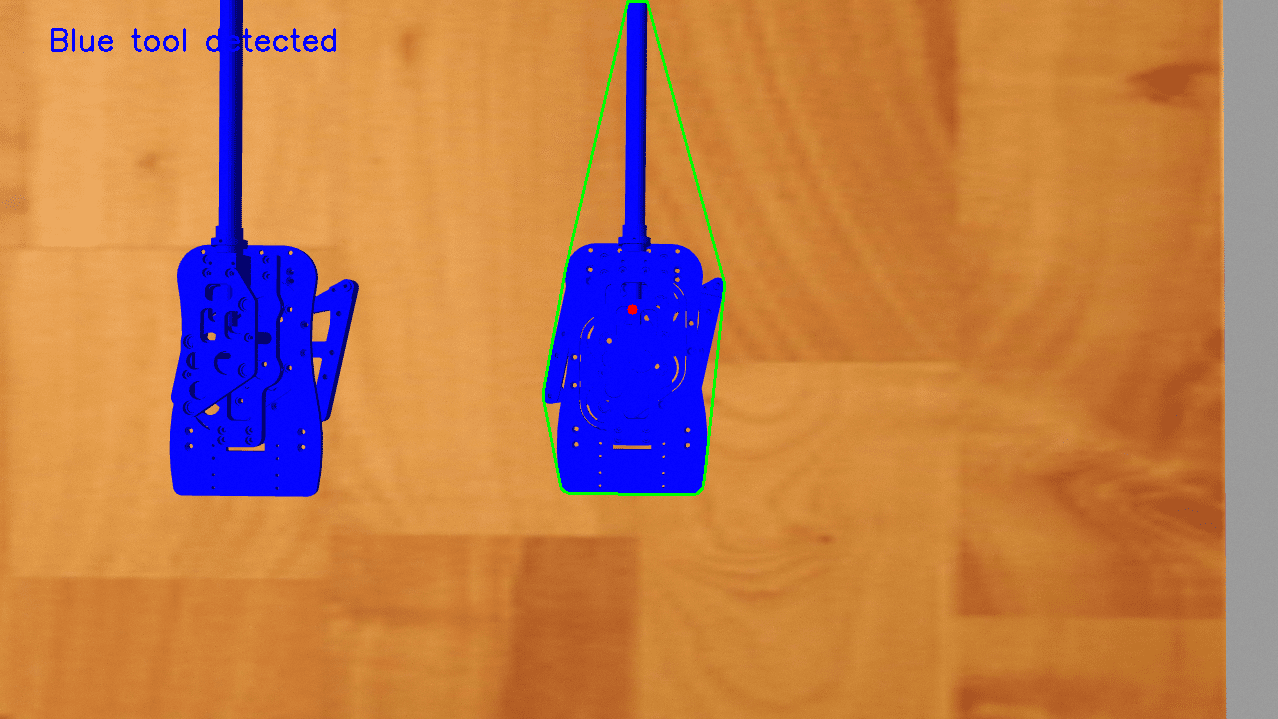
\includegraphics[width=12cm]{images/opencv-tool-convex-hull.png}\\
\caption{Simple tool detection in simulation based on color, using OpenCV. The green polygon is the convex hull, and the red point is the
estimated center of mass}
\end{figure}
\end{center}

\subsection{Stereoscopic vision}

\begin{center}
\begin{figure}[H]
\centering
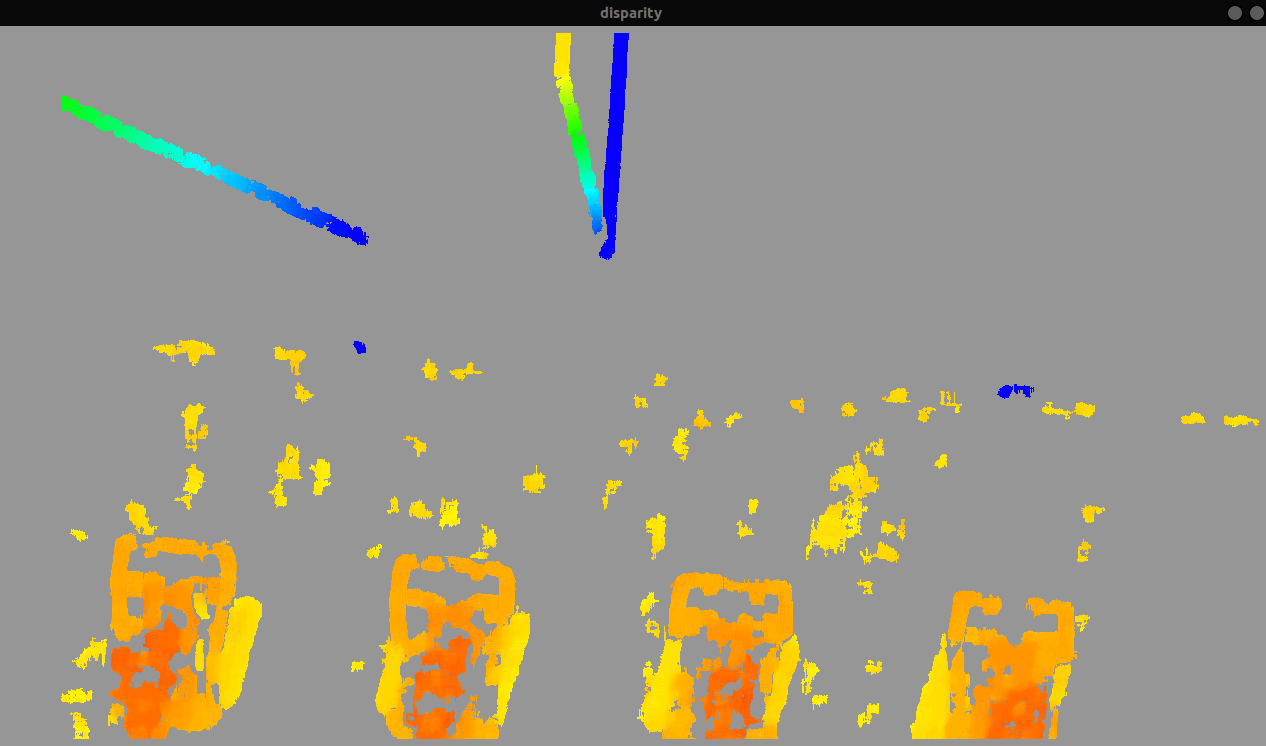
\includegraphics[width=12cm]{images/disparity.png}\\
\caption{Disparity image calculated from the 2 cameras}
\end{figure}
\end{center}

\begin{center}
\begin{figure}[H]
\centering
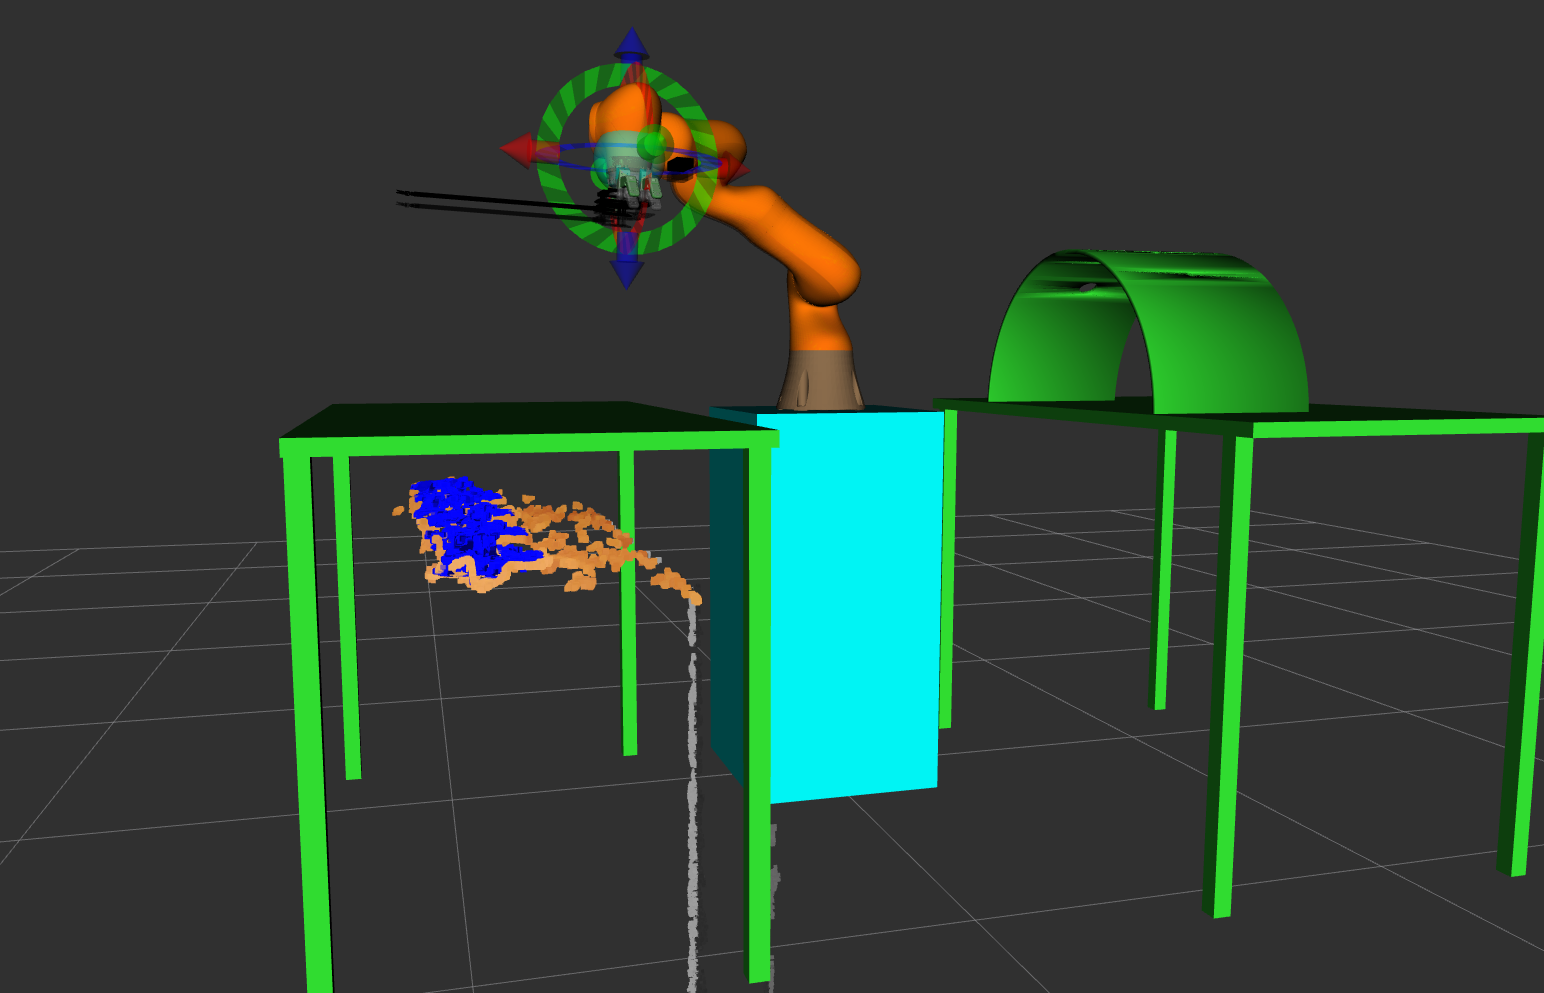
\includegraphics[width=12cm]{images/point_cloud.png}\\
\caption{Point cloud of surgical tools, generated from the 2 cameras and visualized in RViz}
\end{figure}
\end{center}

\subsection{Calculation of tool position and orientation}

In order for the gripper to grasp correctly the laparoscopic tool, it is required to calculate the tool's position and orientation in the pixel space 
which must then be converted with respect to the robot's workspace. From all the pixels that have been classified as part of the laparoscopic tool, 
one can estimate the center of mass and two perpendicular vectors 
attached to that point that define the orientation. The center of mass is simply the average of the $(x,y)$ coordinates of all the tool's pixels
\[
\left( \bar{x}, \bar{y} \right) = \left( \frac{1}{N}\sum_{i=1}^{N} x_i , \frac{1}{N}\sum_{i=1}^{N} y_i \right)
\]
The two orientation vectors are the eigenvectors of the covariance matrix of the above pixels. Let $\mathbf{a},\mathbf{b}$ be the orientation vectors, 
then $\mathbf{a},\mathbf{b}$ are solutions of the equation
\[
C \mathbf{v} = λ \mathbf{v}
\]
where $C$ is the covariance matrix given by
\[
C = \begin{bmatrix}
σ(x,x) & σ(x,y) \\
σ(y,x) & σ(y,y) \\
\end{bmatrix}
\]
\[
σ(x,y) = \frac{1}{n-1} \sum_{i=1}^{N} ( x_i - \bar{x} )( y_i - \bar{y} )
\]

\begin{center}
\begin{figure}[H]
\centering
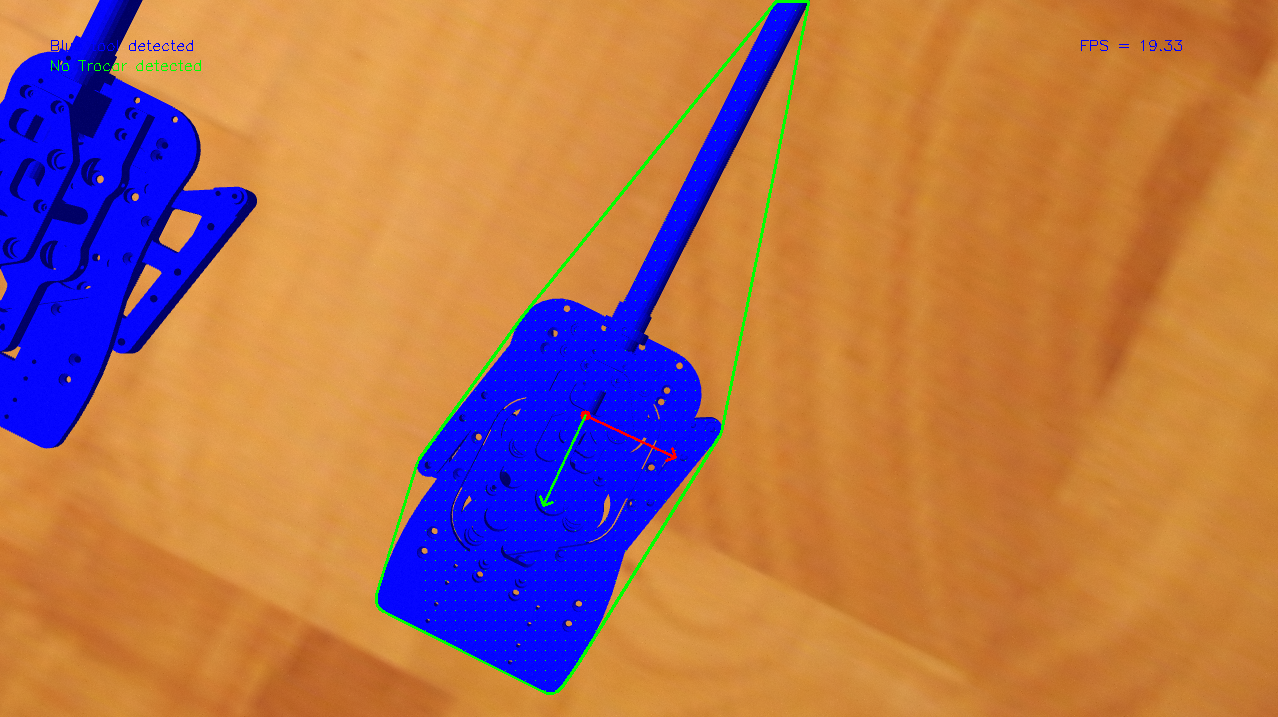
\includegraphics[width=12cm]{images/tool-pose.png}\\
\caption{Estimation of tool's pose (position and orientation)}
\end{figure}
\end{center}

\subsection{Calculation of grasping points}

\subsection{Trocar detection \& Estimation of fulcrum point}

\begin{center}
\begin{figure}[H]
\centering
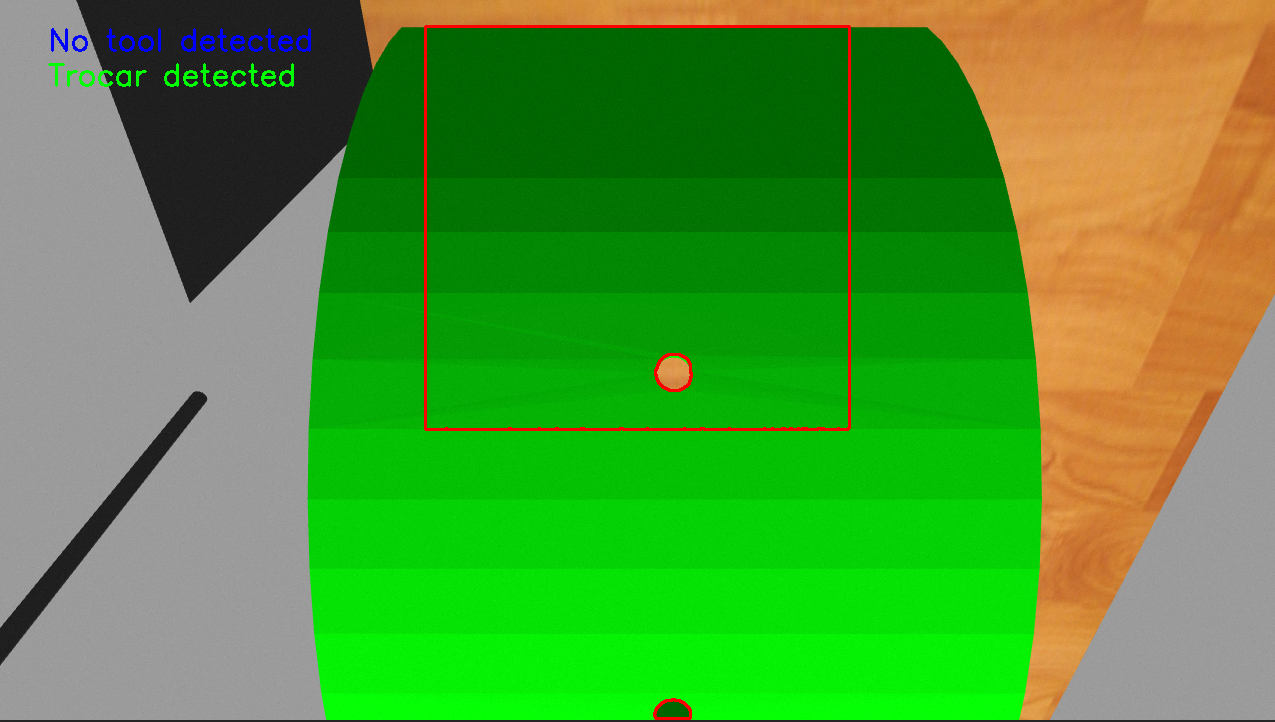
\includegraphics[width=12cm]{images/opencv-trocar-detection.png}\\
\caption{Simple trocar detection in simulation based on color, using OpenCV. In simulation, the trocar is simply considered to be a small 
cylindrical hole and it's center is the fulcrum point}
\end{figure}
\end{center}